\documentclass[tikz,border=0pt]{standalone}
% Deterministic vector typography; formulas are compiled by XeLaTeX.
\usepackage{fontspec}
\IfFontExistsTF{Comic Sans MS}{\setmainfont{Comic Sans MS}}{\setmainfont{texgyreheros}[Extension=.otf,UprightFont=*-regular,BoldFont=*-bold,ItalicFont=*-italic,BoldItalicFont=*-bolditalic]}
\usepackage{amsmath}
\usepackage{fix-cm}
\usepackage{tikz}
\usetikzlibrary{arrows.meta,calc,positioning,shapes.geometric,backgrounds}
\definecolor{ink}{HTML}{2D2730}
\definecolor{muted}{HTML}{716771}
\definecolor{aubergine}{HTML}{563D5D}
\definecolor{coral}{HTML}{D66D75}
\definecolor{sage}{HTML}{7A9E7E}
\definecolor{ochre}{HTML}{C99331}
\definecolor{cream}{HTML}{FFF9F0}
\definecolor{lavender}{HTML}{F1EAF2}
\definecolor{mint}{HTML}{EDF4ED}
\definecolor{blush}{HTML}{FBECEE}
\definecolor{line}{HTML}{DED5DB}
\definecolor{green}{HTML}{4C7B00}
\definecolor{nvidiagreen}{HTML}{76B900}
\definecolor{graphite}{HTML}{242829}
\tikzset{
  every node/.style={font=\fontsize{8}{10.2}\selectfont,text=ink,inner sep=0pt},
  title/.style={font=\bfseries\fontsize{12}{14}\selectfont,anchor=west},
  sub/.style={font=\fontsize{7.5}{9.5}\selectfont,text=muted},
  label/.style={font=\bfseries\fontsize{8.6}{11}\selectfont},
  flow/.style={-{Latex[length=2.1mm,width=1.5mm]},line width=.9pt,draw=aubergine},
  control/.style={-{Latex[length=1.8mm,width=1.3mm]},line width=.8pt,dashed,draw=muted},
  card/.style={rounded corners=2.5mm,draw=line,line width=.65pt,fill=white},
  icon/.style={draw=aubergine,line width=.8pt},
}
\newcommand{\status}[2]{\node[sub,anchor=east,text=#2] at (16.83,#1) {ILLUSTRATIVE $\cdot$ NOT MEASURED};}
\newcommand{\step}[3]{\node[circle,fill=#3,text=white,font=\bfseries\fontsize{8}{8}\selectfont,minimum size=5mm] at (#1,#2) {};}
\newcommand{\thumbnail}[3]{%
  \begin{scope}[shift={(#1,#2)}]
    \fill[fill=#3,draw=aubergine!60,line width=.6pt,rounded corners=.6mm] (0,0) rectangle (1.05,.70);
    \draw[draw=aubergine!55,line width=.7pt] (.12,.15)--(.36,.38)--(.55,.20)--(.77,.46)--(.94,.21);
    \fill[ochre!80] (.23,.53) circle (.065);
  \end{scope}}

\begin{document}
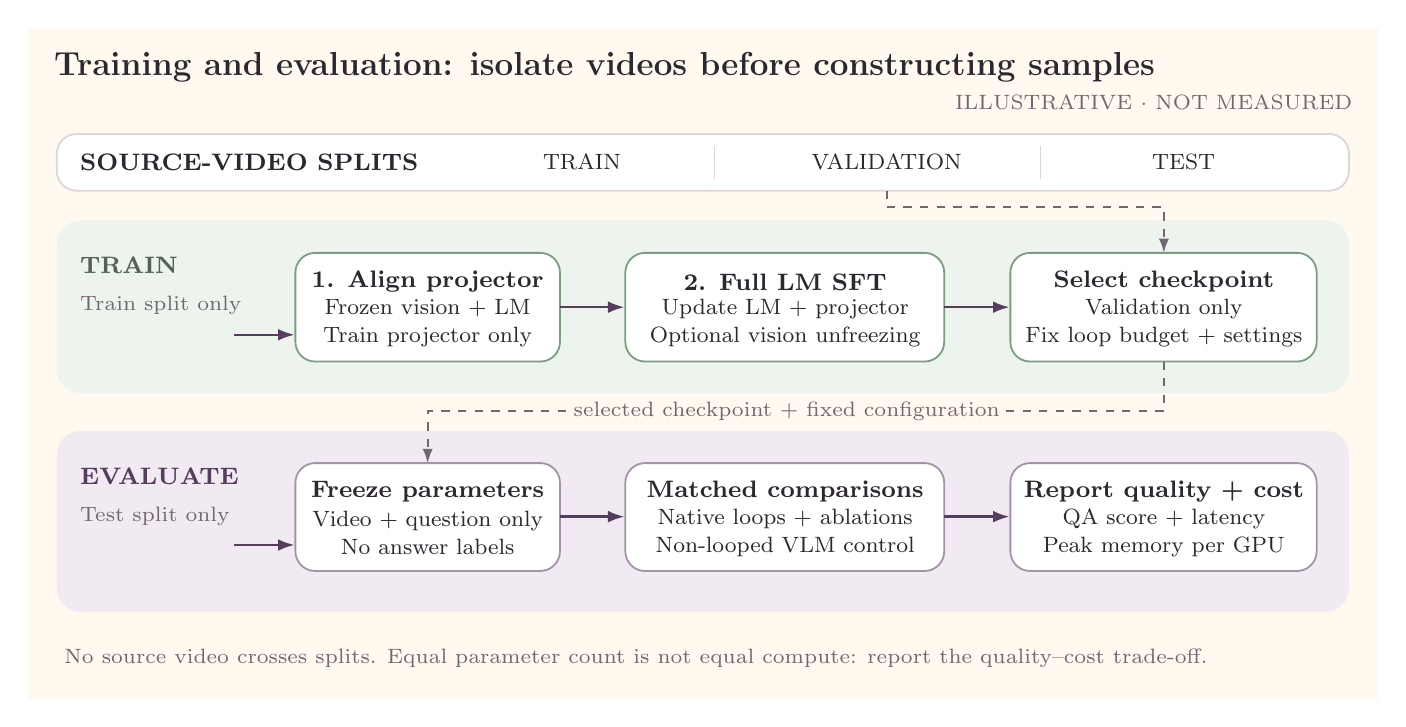
\begin{tikzpicture}[x=1cm,y=1cm]
\path[use as bounding box] (0,0) rectangle (17.145,8.52);
\fill[cream] (0,0) rectangle (17.145,8.52);
\node[title] at (.33,8.02) {Training and evaluation: isolate videos before constructing samples};
\status{7.57}{muted}
\fill[card,fill=white] (.37,6.45) rectangle (16.78,7.17);
\node[label,anchor=west] at (.66,6.81) {SOURCE-VIDEO SPLITS};
\node at (7.04,6.81) {TRAIN};
\node at (10.91,6.81) {VALIDATION};
\node at (14.68,6.81) {TEST};
\draw[line] (8.72,6.60)--(8.72,7.02);
\draw[line] (12.86,6.60)--(12.86,7.02);
% Upper lane: fitting and model selection only.
\fill[rounded corners=3mm,fill=mint] (.37,3.88) rectangle (16.78,6.07);
\node[label,text=sage!50!ink,anchor=west] at (.66,5.50) {TRAIN};
\node[sub,anchor=west] at (.66,5.00) {Train split only};
\fill[card,draw=sage] (3.40,4.28) rectangle (6.76,5.66);
\node[label] at (5.08,5.29) {1. Align projector};
\node[align=center] at (5.08,4.77) {Frozen vision + LM\\Train projector only};
\draw[flow] (2.62,4.62)--(3.39,4.62);
\fill[card,draw=sage] (7.59,4.28) rectangle (11.64,5.66);
\node[label] at (9.62,5.29) {2. Full LM SFT};
\node[align=center] at (9.62,4.77) {Update LM + projector\\Optional vision unfreezing};
\draw[flow] (6.76,4.97)--(7.58,4.97);
\fill[card,draw=sage] (12.48,4.28) rectangle (16.37,5.66);
\node[label] at (14.43,5.29) {Select checkpoint};
\node[align=center] at (14.43,4.77) {Validation only\\Fix loop budget + settings};
\draw[flow] (11.64,4.97)--(12.47,4.97);
\draw[control] (10.91,6.45)--(10.91,6.24)--(14.43,6.24)--(14.43,5.66);
% Lower lane: fixed parameters, test labels used by scorer only.
\fill[rounded corners=3mm,fill=lavender] (.37,1.10) rectangle (16.78,3.40);
\node[label,text=aubergine,anchor=west] at (.66,2.82) {EVALUATE};
\node[sub,anchor=west] at (.66,2.32) {Test split only};
\fill[card,draw=aubergine!55] (3.40,1.62) rectangle (6.76,2.99);
\node[label] at (5.08,2.63) {Freeze parameters};
\node[align=center] at (5.08,2.10) {Video + question only\\No answer labels};
\draw[flow] (2.62,1.95)--(3.39,1.95);
\fill[card,draw=aubergine!55] (7.59,1.62) rectangle (11.64,2.99);
\node[label] at (9.62,2.63) {Matched comparisons};
\node[align=center] at (9.62,2.10) {Native loops + ablations\\Non-looped VLM control};
\draw[flow] (6.76,2.31)--(7.58,2.31);
\fill[card,draw=aubergine!55] (12.48,1.62) rectangle (16.37,2.99);
\node[label] at (14.43,2.63) {Report quality + cost};
\node[align=center] at (14.43,2.10) {QA score + latency\\Peak memory per GPU};
\draw[flow] (11.64,2.31)--(12.47,2.31);
\draw[control] (14.43,4.28)--(14.43,3.65)--(5.08,3.65)--(5.08,2.99);
\node[sub,fill=cream,inner sep=2pt] at (9.64,3.65) {selected checkpoint + fixed configuration};
\node[sub,anchor=west] at (.46,.51) {No source video crosses splits. Equal parameter count is not equal compute: report the quality--cost trade-off.};
\end{tikzpicture}
\end{document}
